%Linea Para poder completar automaticamente las citas con el Sublime
%No hace el documento, se puede borrar esta linea si no se usa el Sublime
%------------------------------------------------------------------------------
 \newcommand{\NoBiblioEQ}[1]{
 \ifthenelse{\equal{#1}{verdadero}}{}{\bibliography{Referencias/base_bibliografica}}
 \NoBiblioEQ{verdadero}}
 %----------------------------------------------------------------------------- 

%Formato (Nombre de capitulo largo o corto), nombre del capitulo y estilo de la
%Portada del Capitulo
%------------------------------------------------------------------------------

 %Formato en si, titulo en un solo renglon
 \FormatoCapituloDosLineas
 
 %Nombre y etiquete para referir
 \chapter{Propiedades de transporte de los sensores}
 \label{chap:Electroquimica}

 %Para que no salga el numero de pagina en la portada del capitulo
 \thispagestyle{empty}
	
 %Resumen del Capitulo en Italica
 \noindent\textit{Aca va todo el desarrollo de la fisicoquimica de los mesospororos, fenomenos de  transporte, adsorcion, lagmuir, propiedades de mediacion redox, catalisis, etc, etc.}

 %Indice de capitulo alineada al borde inferior de la pagina, nueva pagina
 \vfill
 \minitoc
 \newpage
 %-------------------------------------------------------------------------------

\section{Introducción}

	Aca tengo que poner como es la reaccion del punto isoeletrico del Sio2 o del punto de carga zero... o del pka??? Y tambien tengo que poner los antecendente de calvo, calvo y el otro del 2005. Y tambien entonces que la diferencia es el Au miniaturizacion, etc, etc mayores velocidades... etc. 
	No olvidarse de los ferrocenos a distintas velociades de barrido

\section{Adsorcion de sondas, exclusión, permeación y preconcentración}

	Durante las próximas secciones se interpretarán los resultados obtenidos al colocar soluciones con sondas electroquímicas, con diferentes cualidades, sobre los sensores. Al ser,  la fabricación de los sensores, una parte estructural de este trabajo, cabe aclarar sobre que sistemas que se realizaron los resultados de los experimentos que mostraremos durante el desarrollo de este capitulo. Se utilizó, indistintamente, películas de Au sobre sustratos varios (silicio, vidrio, flexible), con diseño ya transferido o sin transferir. Salvo que se aclare lo contrario, se trabajó siempre con sistemas con la película delgada mesoporosa sintetizada con el método de alto vacío (consultar sección \ref{sec:trat-vacio}, pág. \pageref{sec:trat-vacio}). Todas las medidas fueron normalizadas por el área geométrica, de forma de facilitar la comparación cuando se trata de sensores con distinto diseño.  

	\subsection{Exclusión}

	\subsection{Permeación}

	\subsection{Pre-concentración}

\section{Mediacion redox y catalisis}

\section{Modelo propuesto}

\section{Conclusiones parciales}

% 	Aca Hay que poner los graficos de 1mM de Ru para INTI baja T y CNEA calcinado donde se muestra y se pueden vislumbrar los dos mecanismos de transporte de carga, el de libre y el Ru adsorbido.!!!!

% 	Agragar todo lo del ferroceno, lo catalisis con HQ y tambien la mediacion con ferro/ferri

% 	Tambien poner curva de Lagmuir y curvas donse se ve como se disuelve el electrodo! SIEMPRE con cualquier sonda

% 	Aca poner el grafico de estabilidad en funcion del tiempo, explicar que onda que se disuelve pero solo cuando se le hace EQ, que solo aguanta 48 HS.... que no es despegado, etc, etc, que otros sistemas con ITO tambien demostraron los mismos resultados, y que los experimentos siempre terminamos con ferri/ferro para demostrar que la membrana esta intacta.

% 	Preconcentacion, comparacion con calcindado y bajas T
% 	\marginpar{Probar el Au-CTAB en Vacio y calcinado con aminorutenio para ver comportamiento del film, tengo dos muestras buenas que puede servir... la de calcinado es imposible, porque va a dar mal por el AU.}
	

% 	Hay que tener en cuenta aqui el tema de la respuesta Eq que solo son sitios activos los adsorbido y que puede que haya mas Rutenio adsorbido en realiadad. Es una cota inferior de la concentracion dentro de lo poros. Además esta el tema del area, trabajamos siempre con el area geometrica pero se sabe que esta no es el area del electrodo activa sino que es mas..... ambos efectos van en el mismo camino a favor de una mayor concentracion.

% 	\subsection{Medición del espesor y homogeneidad}
			
% 			Ventana de trabajo antes de la solubilidad de las peliculas, porque se disuelven, etc. etc.
			
% 			\subsection{Respuesta electroquímica}
	 		
% 		 		\indent Una vez depositadas las películas bicapa de Cr/Au o de Ti/Au se procedió a evaluar el desempeño electroquímico de las mismas, para poder utilizarlas como electrodos para la fabricación de los sensores. En el capítulo \ref{chap:Materiales} se describe con detalle el montaje experimental para obtener las voltametrías cíclica. Se usaron como sondas electroquímicas ferrocinuro/ferricianuro de potasio (\ferroferri, \fe), cloruro de hexaaminorutenio(III) (\aminorutenio, \ru), hidroquinona (\hidroquinona, \hq) y ferroceno etanol (\ferroceno, \fc). La elección de estas sondas modelos tiene que ver fundamentalmente con la carga neta de cada una de ellas y con la reversibildiad de los pares redox. Analizaremos ahora como fue la respuesta de las películas delgadas de Au para cada una de estas sondas:
		 		
% 		 		\begin{itemize}
		 		 
% 		 		 \item \textit{Respuesta de ferrocinuro/ferricianuro de potasio.}
% 			 		 Se preparó una solución equimolar de \fe\space  para cada una de las concentraciones utilizadas. En electroquímica este par redox es frecuentemente utilizado para evaluar la calidad de los electrodos, ya que es un par redox que se comparta de forma reversible frente al intercambio electrónico electrodo-especie, la reacción que tiene lugar es la siguiente:
% 			 			 %Redox del Ferro/Ferri	 
% 			 			 	 \begin{equation}
% 					 		 \schemestart 
% 					 		 $Fe(CN)_6^{4-}$  
% 					 		 \arrow{<=>[\scriptsize oxidación][\scriptsize reducción]}[0,1.5] 
% 					 		 $Fe(CN)_6^{3-}+e^-$ \schemestop
% 					 		 \end{equation}
% 			 		 Se graficaron diferentes concentraciones de la sonda  a distintas velocidades de barrido para comprobar la respuestas de los electrodos, la cual se espera que siga el comportamiento descrito por Randle-Sevcik, donde \linebreak
% 			 			 %Ecuacion de Randle-sevcik	
% 			 			     \begin{equation}
% 					 		 i_p=0.4463nFAC\left(\frac{nFvD}{RT}\right)^{1/2}
% 					 		 \end{equation}
% 			 		 la intensidad de pico ($i_p$) es proporcional a la concentración ($C$) y a la velocidad de barrido a la $1/2$ $(v^{1/2})$. 
% 			 		 	 %Graficos para el Ferro/Ferri
% 						 		\begin{figure}[ht]
% 						 	    	\begin{subfigure}[t]{0.495\textwidth}
% 						         	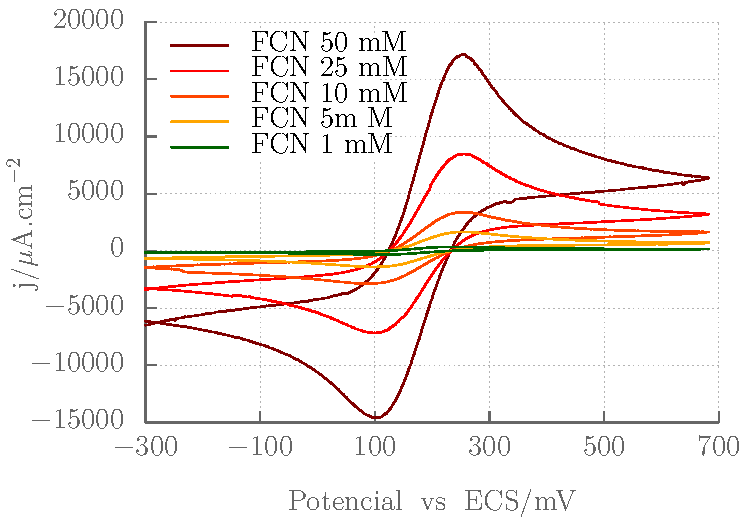
\includegraphics[width=\textwidth]{Graficos/Concentraciones_Fe.pdf}
% 						        	\caption{Voltametrías cíclicas para la cupla \fe\space a diferentes concentraciones, 1mM, 5mM, 10mM, 25mM y 50mM. Todas medidas fueron tomadas a 50mV/s.}
% 						         	\label{fig:Fe_a}
% 						     		\end{subfigure}
% 					     		 \begin{subfigure}[t]{0.495\textwidth}
% 						        	\includegraphics[width=\textwidth]{Graficos/Calibracion_Fe.pdf}
% 						       		\caption{Curva de calibración para distintas concetraciones de la cupla \fe\space valores tomados de la \ref{fig:Fe_a}.}
% 						         	\label{fig:Fe_b}
% 						     		\end{subfigure}
% 						     		%\vspace*{0.5cm}

% 					 	     	\begin{subfigure}[t]{0.495\textwidth}
% 					         		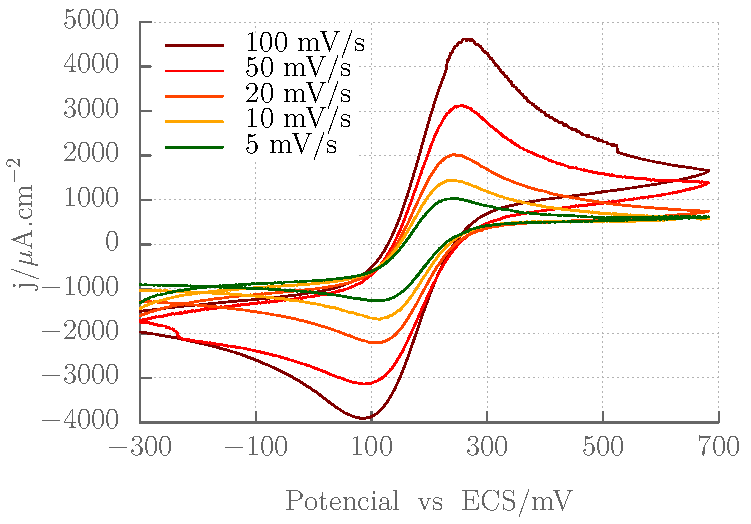
\includegraphics[width=\textwidth]{Graficos/Velocidades_Fe.pdf}
% 					        	    \caption{Voltametrías cíclicas de una solución 10mM de la cupla equimolar \fe\space a diferentes velocidades de barrido, 5mV/s, 10mV/s, 20mV/s, 50mV/s y 100mV/s.}
% 					        	    \label{fig:Fe_c}
% 					     		 	\end{subfigure}
% 					     	 	\begin{subfigure}[t]{0.495\textwidth}
% 					        		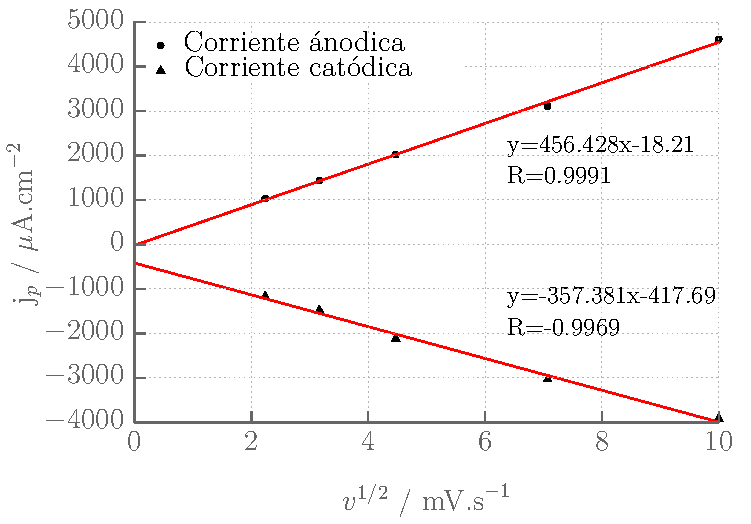
\includegraphics[width=\textwidth]{Graficos/VelocidadesCal_Fe.pdf}
% 					       			\caption{Respuesta frente a diferentes velocidades de barrido para una solución de \fe\space equimolar 10mM, se ve una dependencia lineal con la velocidad a la potencia $1/2$.}
% 					         		\label{fig:Fe_d}
% 					     			\end{subfigure}
% 					     		 \caption{a) Respuesta electroquímica de la cupla equimolar \fe\space para distintas concetraciones, b) curva de calibrado para dichas concentraciones. c) dependencia de la intensidad con la velocidad de barrido y, d) se observa la dependencia lineal con la inversa de la raíz cuadrada de la velocidad de barrido. Todos los voltagramas fueron tomadas con un contraelectrodo de Pt y en una solución 0,1M de NaCl como electrolito soporte.}
% 					     		 \label{fig:ferro-ferri-CV}
% 					     		 \end{figure}

% 			 		 Con estos mediciones demostramos a su vez, que el sistema responde a un proceso de difusión lineal semiinfinita, lo cual era lo que se esperaba para un sistema simple en el que el electrodo esta embebido en la solución soporte (0,1mM KCl, $pH=5.5$) con la sonda electroquímica.
	 		 			 
	 		 	 
% 	 		 	 \item \textit{Respuesta del cloruro de hexaaminorutenio(III).}
% 	 		 	 	 Otra sonda electroquímica de suma importancia que se utilizó durante la tesis fue el cloruro de hexaaminorutenio(III). En solución se disocia para formar el complejo \aminorutenio. La reacción redox que tiene lugar es la siguiente:
% 	 		 	 	 	%Ecuacion redox del aminorutenio
% 	 		 	 	 		\begin{equation}
% 	 		 	 	 			\schemestart 
% 					 			 $Ru(NH_3)_6^{2+}$  
% 					 			 \arrow{<=>[\scriptsize oxidación][\scriptsize reducción]}[0,1.5] 
% 					 		 	 $Ru(NH_3)_6^{3+}+e^-$ \schemestop 
% 	 		 	 	 		\end{equation}
% 	 		 	 	 Dicho par redox, al igual que el \fe\space, responde a un proceso electroquímico reversible, en el cual podemos fácilmente reducir u oxidar el complejo variando el potencial de la solución. Habiendo ya comprobado el correcto desempeño de los electrodos y que cumple con las condiciones de un proceso de difusión semiinfinita, se graficaron varias concentraciones de la sonda para realizar la curva de calibración correspondiente.
% 						%Graficos para el Rutenio
% 						 		\begin{figure}[ht]
% 						 	     \begin{subfigure}[t]{0.495\textwidth}
% 						         	\includegraphics[width=\textwidth]{Graficos/Concentraciones_Ru.pdf}
% 						        	\caption{Voltametrías cíclicas para \ru\space a diferentes concentraciones, 6.3mM, 3.15mM, 1.575mM, 0.63mM y 0.315mM.}
% 						         	\label{fig:Ru_a}
% 						     		\end{subfigure}
% 					     		 \begin{subfigure}[t]{0.495\textwidth}
% 						        	\includegraphics[width=\textwidth]{Graficos/Calibracion_Ru.pdf}
% 						       		\caption{Curva de calibración para la especie \ru. Los valores fueron tomados de la figura \ref{fig:Ru_a}.}
% 						         	\label{fig:Ru_b}
% 						     		\end{subfigure}
% 						     		\label{rutenio}
% 						     		\caption{a) Voltametrías cíclicas para soluciones de \ru\space de distinta concetración y, b) curva de calibración para dichas concentraciones. Todos los voltagramas fueron tomadas a 50mV/s. con contraelectrodo de Pt y en una solución 0,1M de NaCl como electrolito soporte.}
% 						     	 \end{figure}
	 		 	 
% 	 		 	 \item \textit{Respuesta del ferroceno metanol.}
% 	 		 	 	 El \fc\space fue otra de las sondas electroquímicas que se utlizó, su forma reducida tiene carga neutra pero su forma oxidaF	da es positiva. La reacción es la siguiente:
% 	 		 	 	 			%Ecuación redox para el Ferroceno
% 		 	 	 				 \begin{equation}
% 	 		 	 	 				\begin{aligned}
% 	 		 	 	 				\includegraphics[scale=0.65]{Esquemas/Redox-Fc.pdf}
% 	 		 	 	 				\end{aligned}
% 	 		 	 	 			 \end{equation}
% 	 		 	 	 se eligió esta sonda fundamentalmente por la reversibilidad del par redox, y la carga neutra de la forma reducida. La \ref{Fig:Fc} muestra la respuesta electroquimica sobre un electrodo de Au.
% 	 		 	 				%Graficos para el Ferroceno
% 						 		 \begin{figure}[ht]
% 						 	      \begin{subfigure}[t]{0.495\textwidth}
% 						          	\includegraphics[width=\textwidth]{Graficos/Concentraciones_Fc.pdf}
% 						         	\caption{Voltametrías cíclicas para \fc\space a diferentes concentraciones, 1mM, 5mM y 10mM.}
% 						          	\label{fig:Fc_a}
% 						      		\end{subfigure}
% 						      	 \begin{subfigure}[t]{0.495\textwidth}
% 						          	\includegraphics[width=\textwidth]{Graficos/Concentraciones_Fc.pdf}
% 						         	\caption{Curva de calibración para la especie \fc. Los valores fueron tomados de la figura \ref{fig:Fc_a}.}
% 						          	\label{fig:Fc_b}
% 						      		\end{subfigure}
% 						      	 \caption{a) Voltametrías cíclicas para soluciones de \fc\space de distinta concetración y, b) curva de calibración para dichas concentraciones. Todos los voltagramas fueron tomadas a 50mV/s. con contraelectrodo de Pt y en una solución 0,1M de NaCl como electrolito soporte.}
% 						      	 \label{Fig:Fc}
% 					      		 \end{figure}

% 	 		 	 \item \textit{Respuesta de la hidroquinona.}
% 	 		 	 	 La \hq\space a diferencia de las otras sondas que se utilizó durante la tesis tiene dos características diferenciales; una es que tanto la forma oxidada como reducida no tienen carga neta (a lo largo de la tesis se desarrollará el concepto de sonda modelo cargada/neutra para demostrar la permeoselectividad de las membranas),  y la otra es que es el procesos de oxidación de la hidroquinona en benzoquinona y su proceso inverso de reducción son irreversibles.La reacción redox que tiene lugar es la siguiente:
% 	 		 	 \end{itemize}
% 	 		 	 	  			%Ecuacion redox de la HQ
% 	 		 	 	 				\begin{equation}
% 	 		 	 	 				\begin{aligned}
% 	 		 	 	 				\includegraphics[scale=0.65]{Esquemas/Redox-HQ.pdf}
% 	 		 	 	 				\end{aligned}
% 	 		 	 	 				\end{equation}
% 	 		 	 	 			%Graficos para la HQ
% 						 			\begin{figure}[ht]
% 						 	     \begin{subfigure}[t]{0.495\textwidth}
% 						         	\includegraphics[width=\textwidth]{Graficos/Concentraciones_HQ.pdf}
% 						        	\caption{Voltametrías cíclicas para \hq\space a diferentes concentraciones, 1mM, 5mM y 10mM.}
% 						         	\label{fig:HQ_a}
% 						     		\end{subfigure}
% 					     		 \begin{subfigure}[t]{0.495\textwidth}
% 						        	\includegraphics[width=\textwidth]{Graficos/Calibracion_HQ.pdf}
% 						       		\caption{Curva de calibración para la especie \hq. Los valores fueron tomados de la figura \ref{fig:HQ_a}.}
% 						         	\label{fig:HQ_b}
% 						     		\end{subfigure}
% 						     	 \caption{a) Voltametrías cíclicas para soluciones de \hq\space de distinta concetración y, b) curva de calibración para dichas concentraciones. Todos los voltagramas fueron tomadas a 50mV/s. con contraelectrodo de Pt y en una solución 0,1M de NaCl como electrolito soporte.}
% 					     		 \label{fig:HQ}
% 					     		 \end{figure} 
% 				 En la tabla \ref{tabla:sondas} se resumen las características y resultados de las voltametrías cíclicas de cada una de las sondas modelos elegidas. Durante todo el desarrollo de la tesis se utilizaron estos resultados comparar las voltametrías sobre los electrodos desnudos y sobre los electrodos con la película mesoporosa.
% 				  %Tabla resultados EQ
% 				     \begin{table}[ht]
% 			  		  \caption{Resultados y características de las sondas electroactivas utilizadas.}
% 			  		  \begin{tabular}{lccc}\toprule
% 					  Sonda 		& \multicolumn{1}{l}{\hspace{.5cm}Carga especie}\hspace{.5cm} & \multicolumn{1}{l}{\hspace{.5cm}Carga especie}\hspace{.5cm} &\multicolumn{1}{l}{$\Delta$E(mV)}\\
% 					     		    & \multicolumn{1}{l}{\hspace{.5cm}Reducida}      & \multicolumn{1}{l}{\hspace{.5cm}Oxidada}      &    						     \\ \midrule
% 			    	  \ferroferri	& \multirow{1}{*}{$4-$}  		& $3-$								   &  150 		  					 \\ \midrule
% 			  		  \aminorutenio & $2+$							& $3+$								   &  80      						 \\ \midrule
% 			  		  \raisebox{-.5\height}{\includegraphics[scale=0.4]{Esquemas/Fc.pdf}}   &  0 &     1+      &  103 			                 \\ \midrule
% 			  		  \raisebox{-.5\height}{\includegraphics[scale=0.4]{Esquemas/HQ.pdf}}	&  0 &     0       &  Irreversible	 				 \\ 
% 			  		  \bottomrule
% 			    	  \end{tabular}
% 			   		  \label{tabla:sondas}
% 			   		  \end{table}
			   		

% 				 Una vez fabricadas las películas delgadas de Au y determinada la respuesta electroquímica se mostrará en la próxima sección los resultados de sintetizar sobre electrodos de Au películas delgadas mesoporosas de oxido de silicio.

	 		 	
	 		
% 	 		\marginpar{\color{red}Experimentos que falta: Varios puntos para el ferroceno etanol y la curva de calibracion}

	
% \section{Películas mesoporosas}


% \section{Electroquimica de tratamiento con Vacio.}

% CV para demostrar que anda joya comparada con el Au de CNEA calcinado

% \subsection{Síntesis de la película activa}

% 		 		\indent Esta etapa del trabajo involucró la síntesis por sol-gel de películas delgadas de óxido de silicio mesoporoso. Los sensores están compuestos por tres elementos estructurales, el sustrato (silicio, vidrio, polímeros), los electrodos de Au y sobre ellos la <<película activa>>. Esta última es la que se encargará de atribuirle propiedades diferenciales a cada electrodo de cada arreglo de sensores. Como se explico con anterioridad, se escogió oxido se silicio entre otras cosas por su rica diversidad química, por ser transparente en el UV/VIS, por ser un óxido de uso frecuente en microelectrónica y por su bajo costo.

% 	\subsection{Películas delgadas de silica mesoporosa}

% 				\indent Las peliculas fueron depositas por <<spin coating>> 80uL, 4000RPM

% 	\subsection{Caractización}
% 	comparaciones con el ITO, porque usamos Au. adherencia.

% 				Aca va todas imagenes de elipsoporosimetria ambiental para el calcinado. tambien SEM y FIB. y FTIR,



%    Una  

%    Preparación de los soles
% 	Deposito de mesoporosos sobre el Au. Problema de adherencia. Condiciones experimentales, grafico de curva de aceleracion spincoating

% \section{Mediciones electroquímicas}

% Es aqui cuando surgen las primeras incognitas. Un breve introduccion a como se hiceron las mediciones y sobre que sistemas.

% \subsection{Incompatibilidad de los tratamientos térmicos}

% Aca va todo el chorro del Au, del cambio de target, etc, etc. Tabla con todos los experimentos hechos, cambio de agua de las soluciones, cambio de electrolito sporte, cambio de sustrato, sin capa adherente.
% Caracterización electroquímica, problemas, difusión, XPS, etc. ademas de medicdas de ACV? CV? Au de la CNEA, etc. ademas de la resistencia a la trasferencia de electronico. curvas a mas achatadas.

% \subsection{Soluciones a los problemas de Incompatibilidad}

% Cambio en el tarjet de Au, aca van las medidas electroquimicas de Au sobre el target de la CNEA y el del INTI calcinados

% Cambio por ITO, porque si porque no

% Cambio en el tratamiento termico de la sintesis de los mesoporosos a baja T




% Aca va el cambio de au vs tratamientos de bajas temperaturas y aplicable a nuevos sustratos y por supuesto mucho mas economico (por el Au).
% \section{Modelo}

